\section{Edge Intelligence}

State-of-the-art \gls{dnn} are getting deeper i.e. adding more layer to the models to improve model accuracy, however the added amount of model parameters require additional computations, hence inference time is degraded \cite{bibid}. Conventionally intelligent mobile applications have been run in the cloud, introducing highly unreliable latency in \gls{wan}. As end-devices have become more powerful, smaller albeit less accurate \gls{ai} architectures have been proposed, however with the emergence of \gls{iot} less powerful devices, not able to run highly demanding algorithms are constantly being connected to the internet. Devices which work in application, that advantageously could benefit from intelligence. In order to find the right balance between primarily highly accurate \gls{mcc} and highly responsive mobile computing, a new computing paradigm emerges namely \gls{mec}.  

The survey \citetitle{zhou_edge_2019} by \citet{zhou_edge_2019} review the current state within the research field of \gls{ei}. The survey includes training and inference of \gls{dnn} on the edge and categorizes several performance metrics for \gls{ei} applications and services. 

This thesis mainly focuses on the inference process and will not address edge-specific training methods. In these next sections architectures, performance metrics and enabling technologies for edge-centric inference will be described.  

\subsection{Architectures}

Inference architectures for edge-centric \gls{ei} application and services can be categories into four main models \cite{zhou_edge_2019}:

\begin{figure}
	\centering
	\captionsetup[subfigure]{justification=centering}
	\subfloat[Device-based\label{fig:device-based}]{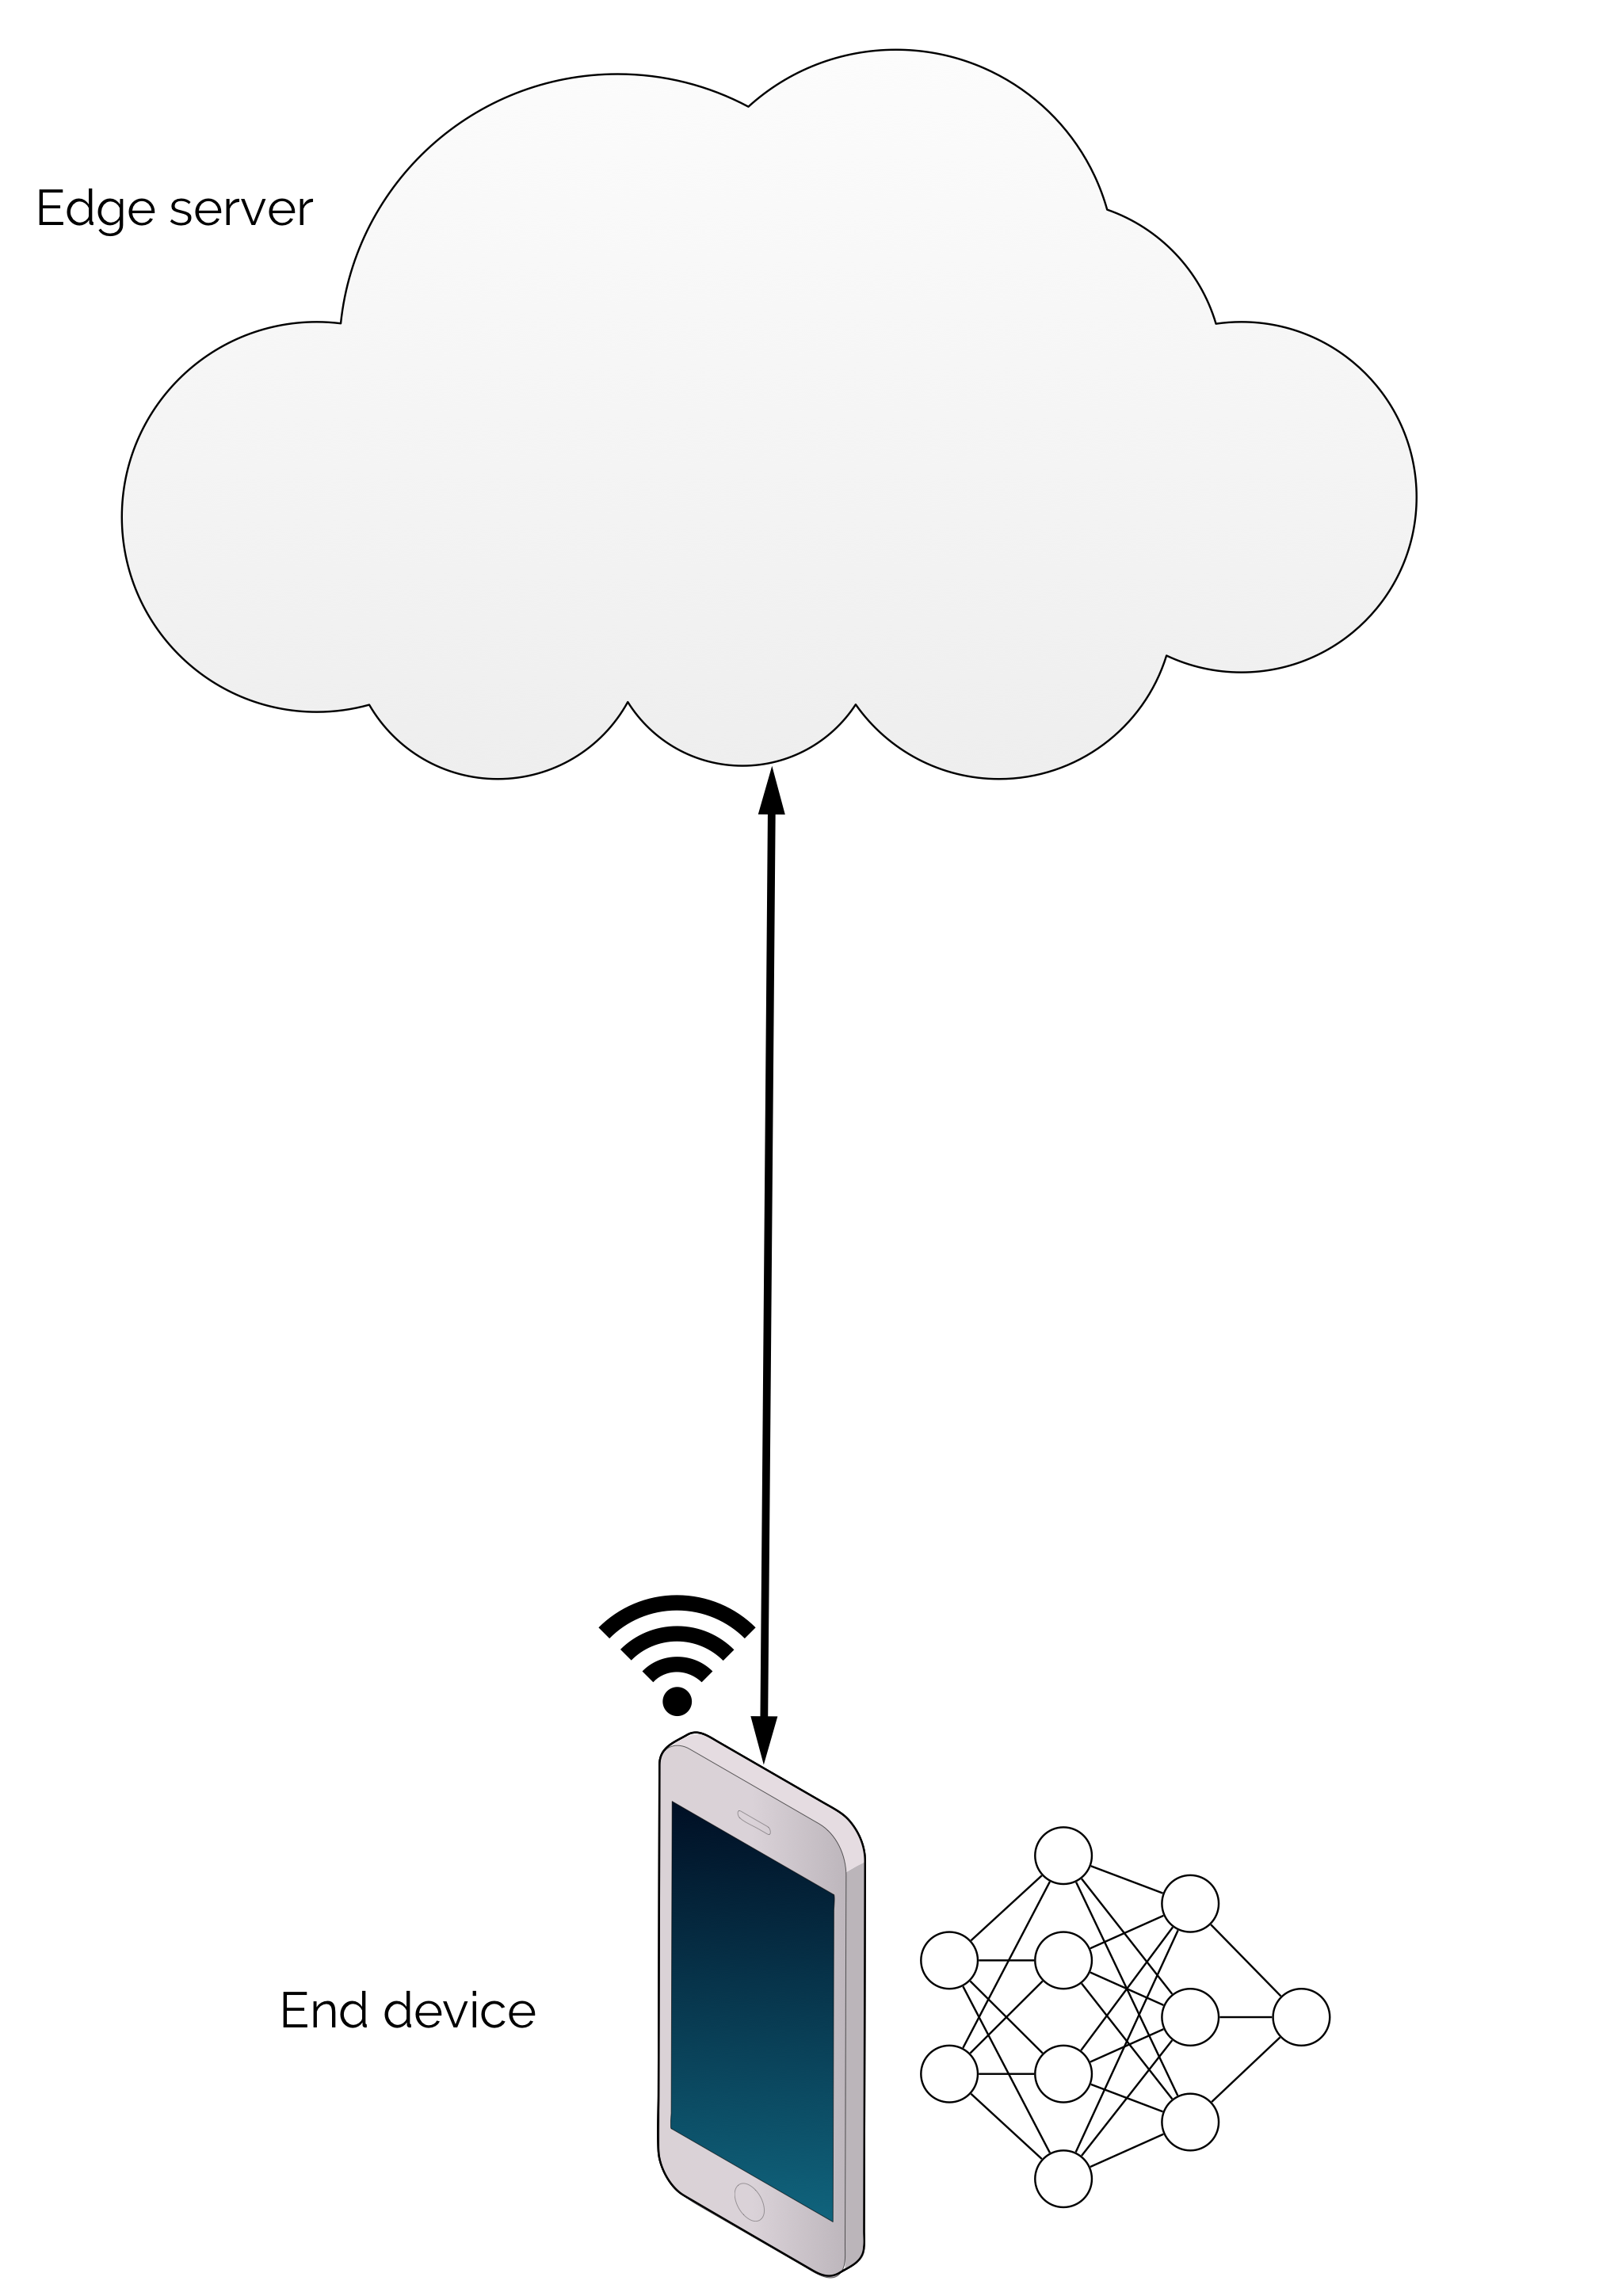
\includegraphics[width=.2\linewidth]{figures/models/device}}
	\subfloat[Edge-based]{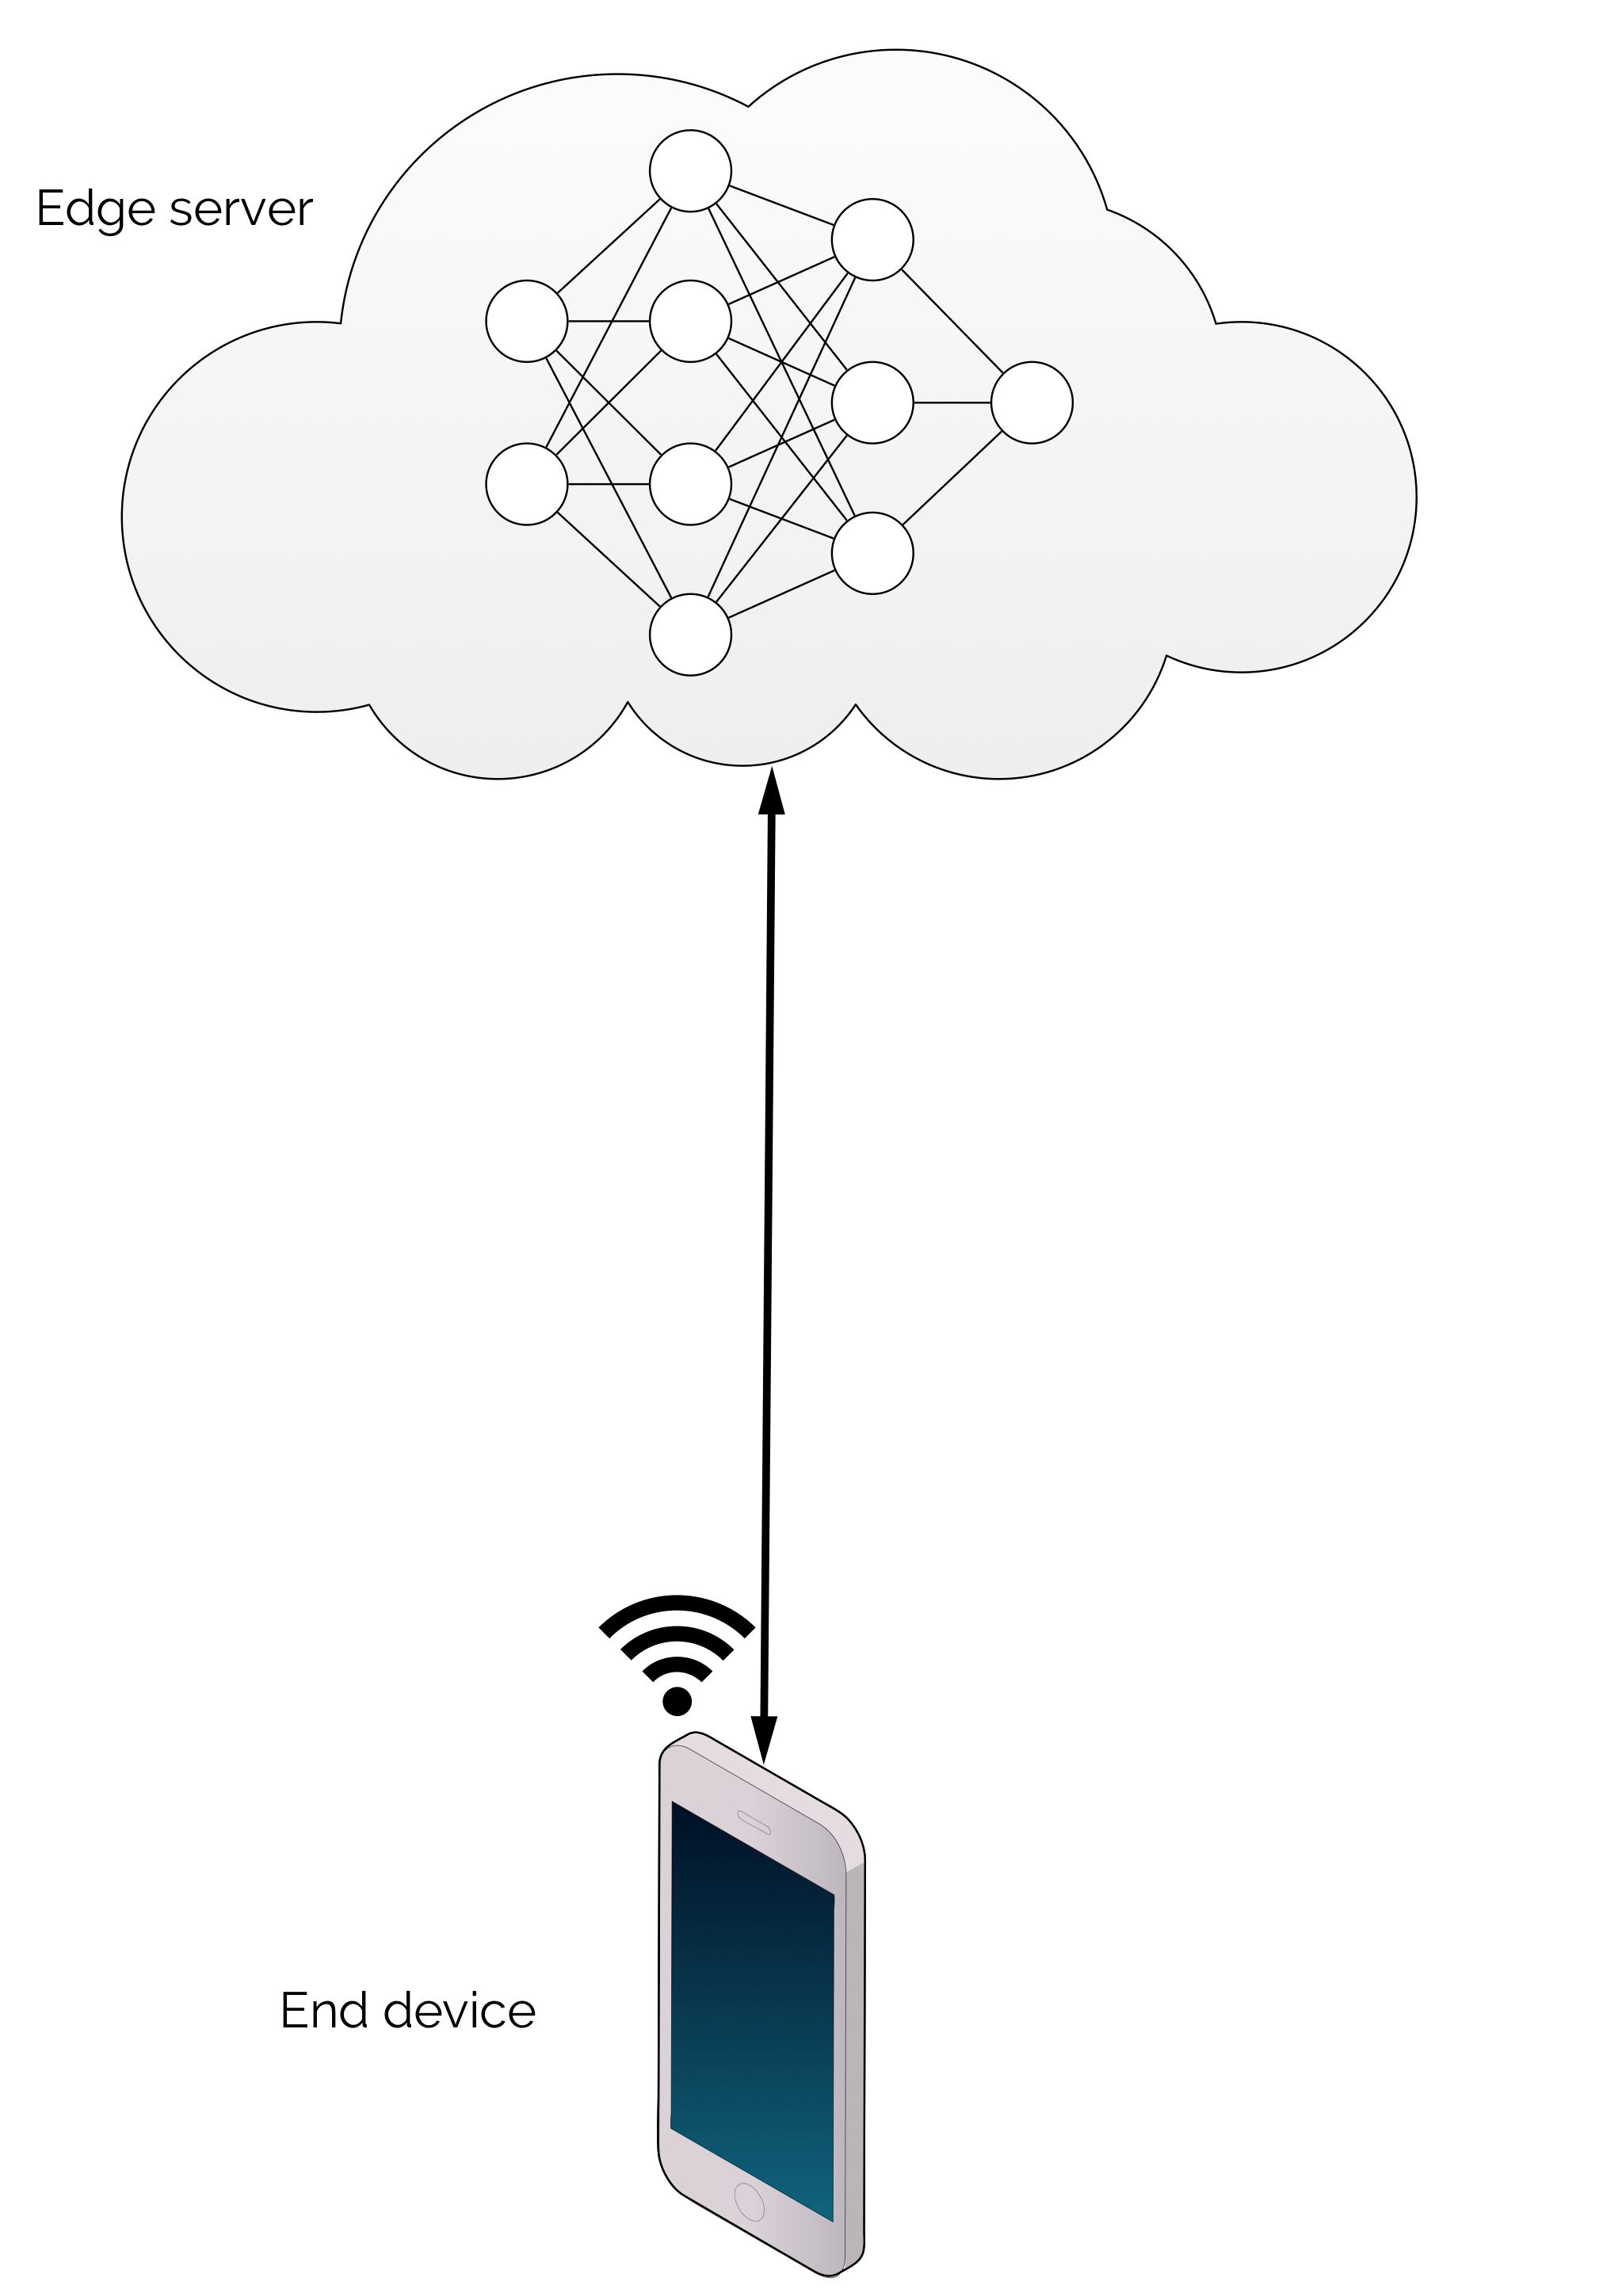
\includegraphics[width=.2\linewidth]{figures/models/edge}}
	\subfloat[Edge-Device mode]{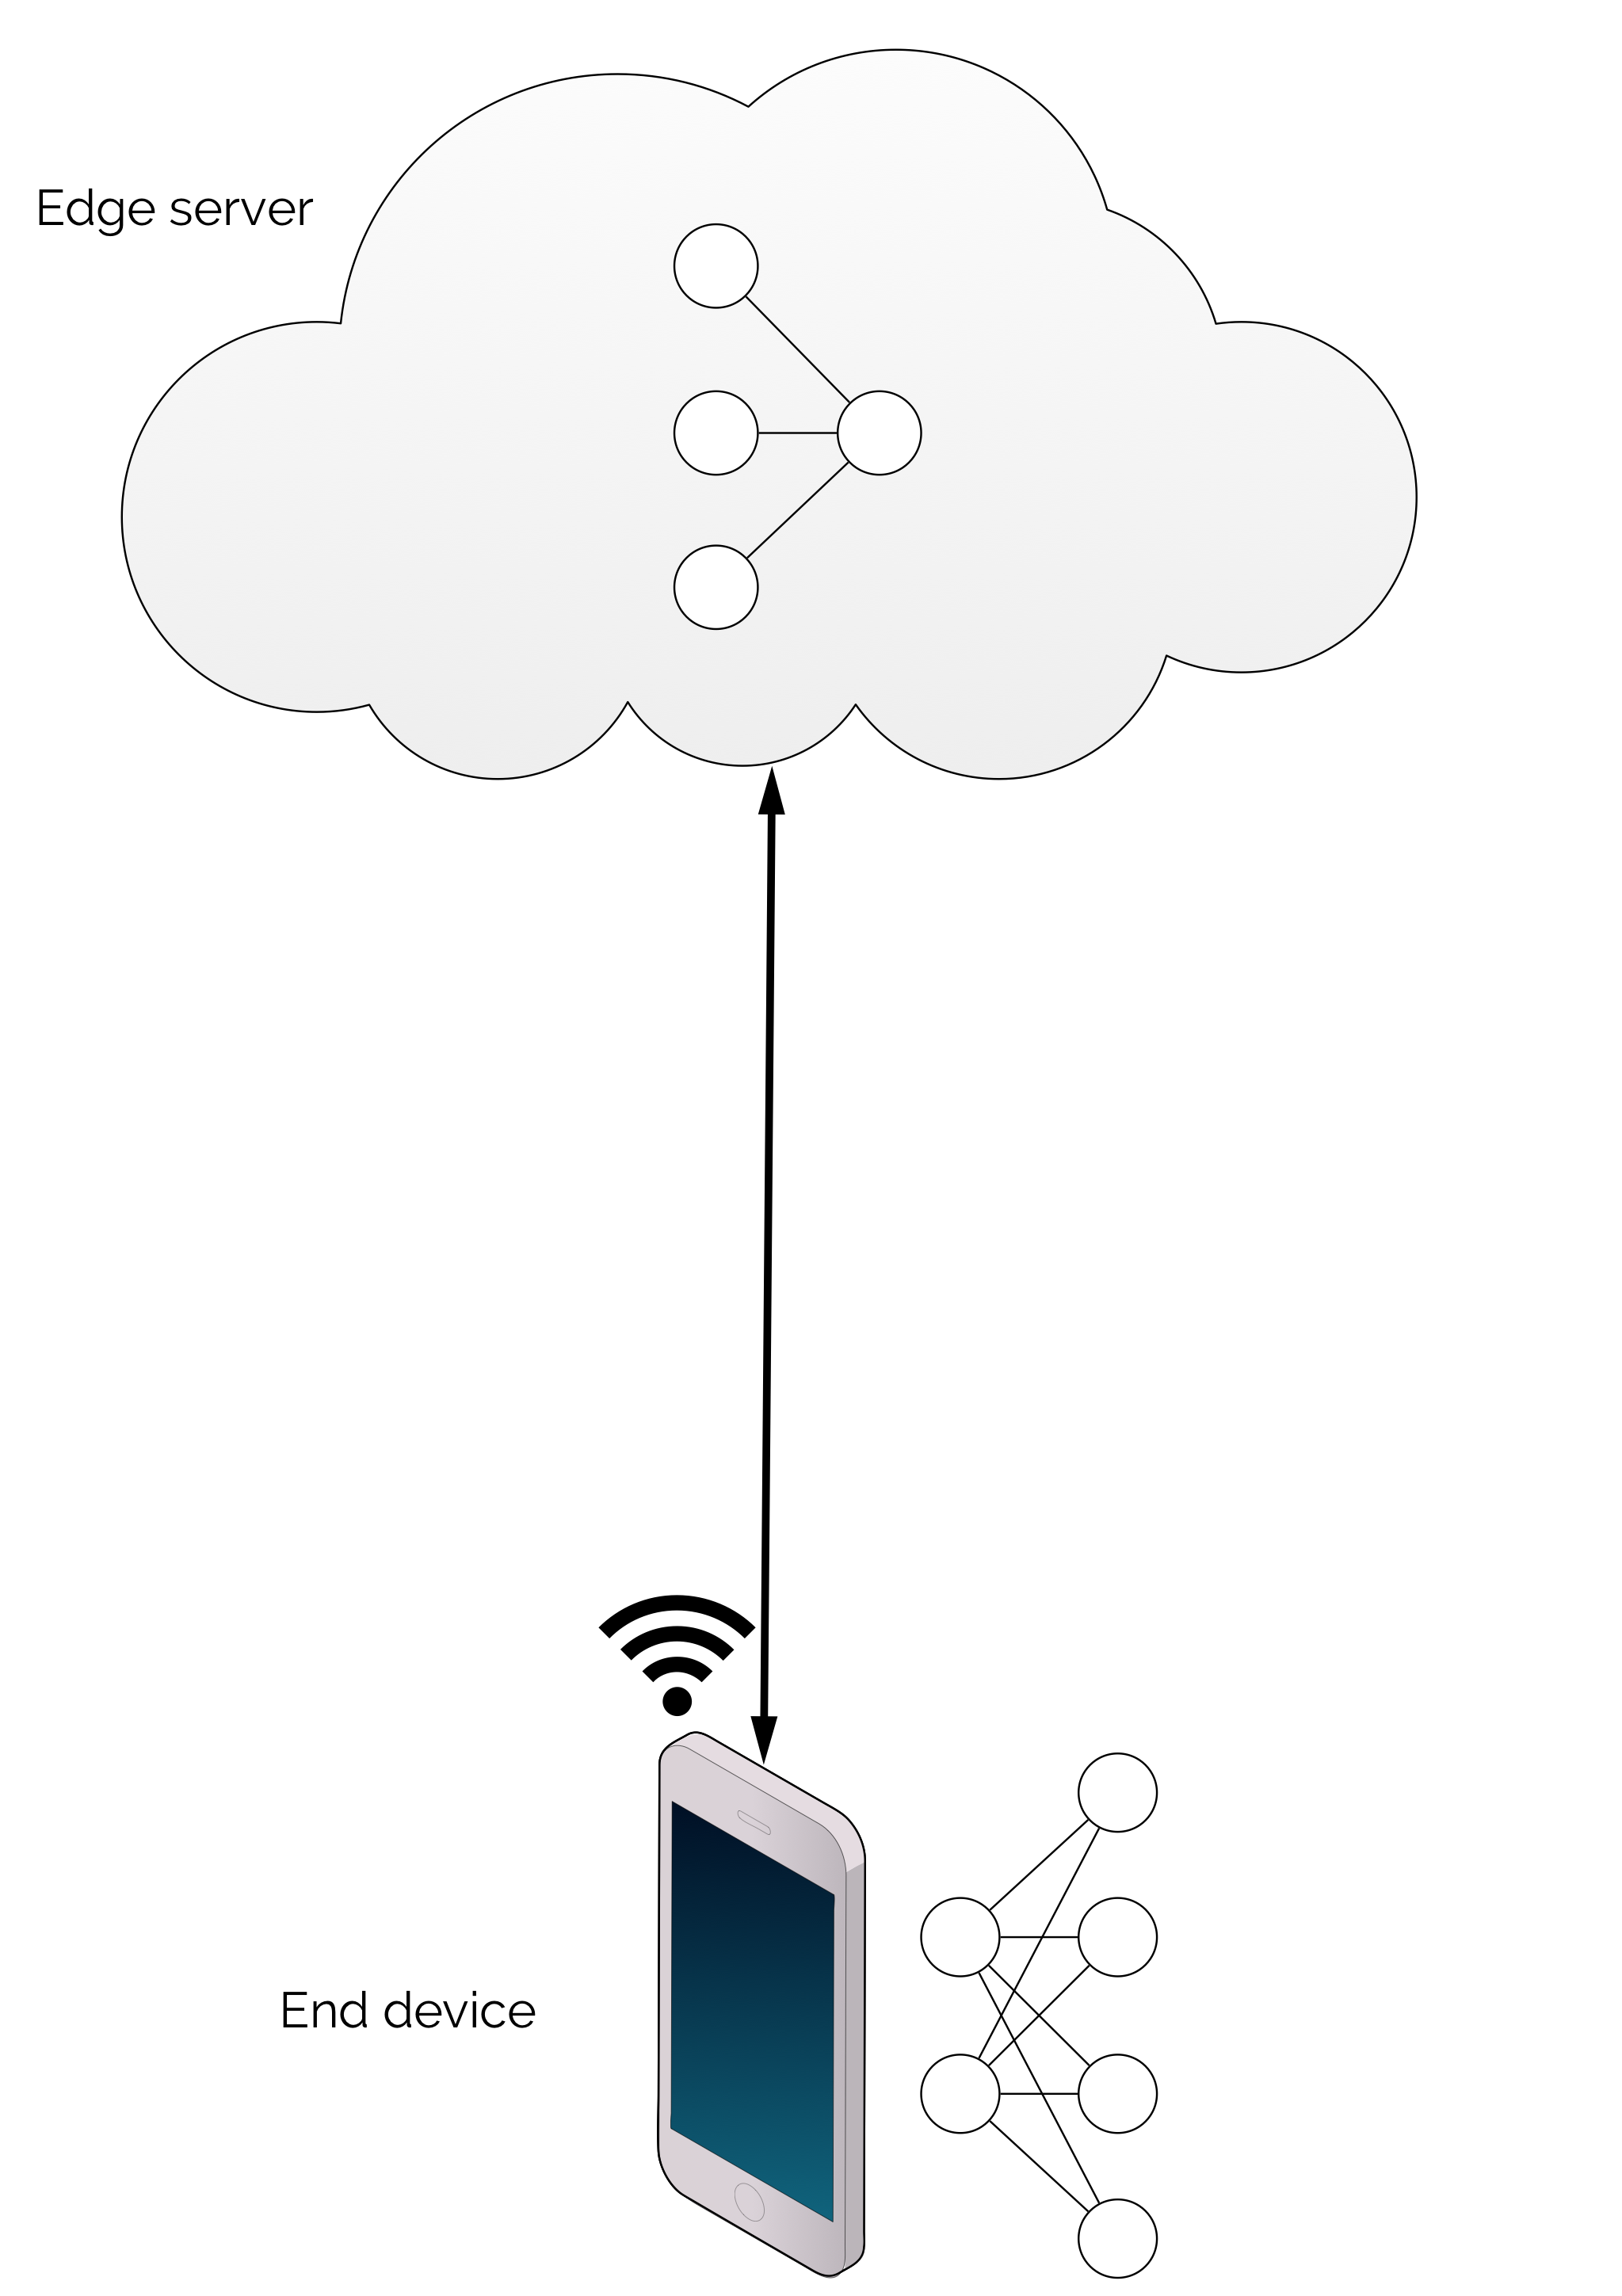
\includegraphics[width=.2\linewidth]{figures/models/edge_device}}
	\subfloat[Edge-Cloud mode]{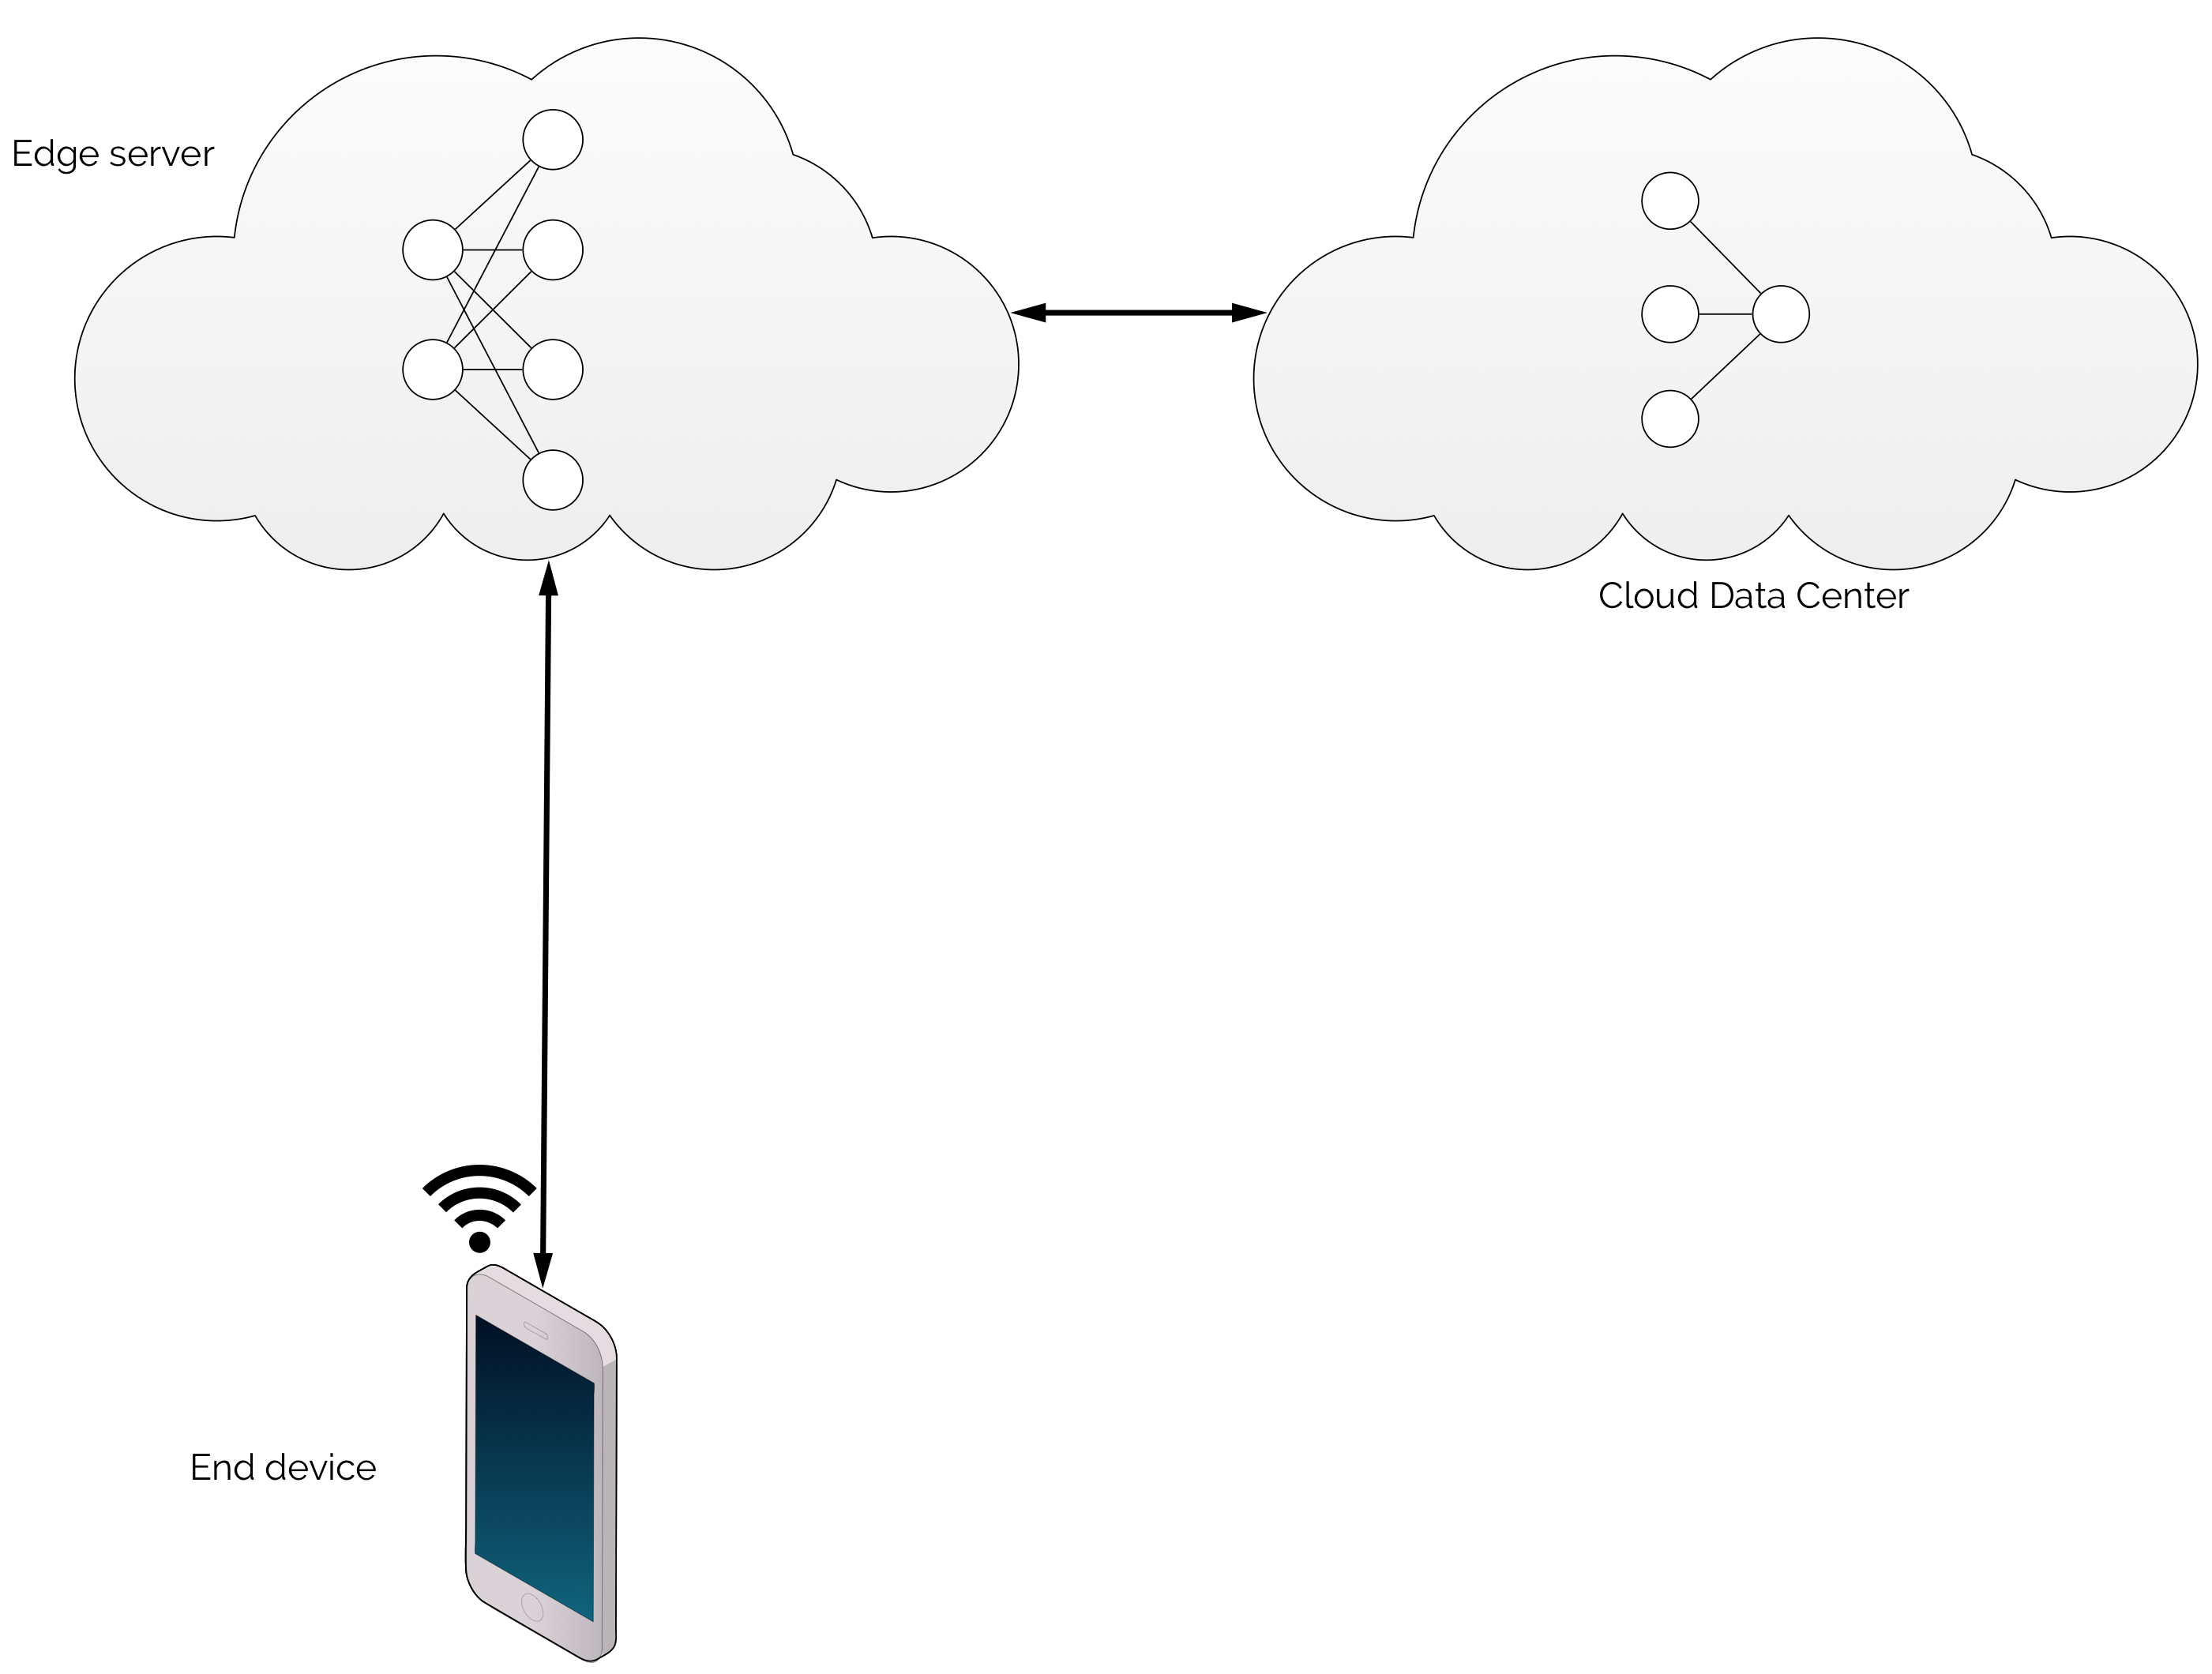
\includegraphics[width=.37\linewidth]{figures/models/edge_cloud}}
	\caption{Edge Archtitectures: \protect\subref{fig:device-based}}
\end{figure}

\begin{description}
	\item[Device-based Mode] end device obtain model from edge server. The end-device then acquires input data and performs model inference. Since all computation is done on the end device, performance is solely reliant on the end device's computing resources.  
	\item[Edge-based Mode] end device acquires input data. The input data is transferred to an edge server, which performs model inference and send the prediction results to the end device. The performance relies on edge server computing resources and network bandwidth.
	\item[Edge-Device Mode] end device acquires input data and performs partially model inference. The intermediate data is transferred to an edge server which finalizes model inference. The performance relies on end device's and edge server computing resource, network bandwidth and edge server workload. 
	\item[Edge-Cloud Mode] resemble edge-device mode, however the model inference task is now partitioned between edge server and cloud data centers. The model is now reliant on edge server and data center computing resources, but even more reliant on \gls{wan} transmission rate between edge and cloud. 
\end{description}

\subsection{Performance Metrics}

The aim of edge intelligence is to accommodate certain performance metrics:

\begin{description}
	\item[Latency] is defined as the overall time of the inference process, including from data is generated at the device, data transmission, preprocessing, model inference and postprocessing. For \gls{ei} real-time application, such as \gls{ar}/\gls{vr}, where stringent deadlines requirements must be met e.g. 100ms. Latency is affected by several factors; computing resources, data rate, model architecture and execution.
	
	\item[Accuracy] is defined as the ratio correctly predicted input samples from the total number of inputs. 
	\begin{align*}
		\alpha = \frac{n_c}{N}
	\end{align*}
	Accuracy requirements are dependent on the \gls{ei} application, for instance autonomous vehicles require extreme accuracy with extremely low latency. The essential trade-off is how accurate a model can we use while still satisfying latency demands.  
	
	\item[Energy efficiency] is important as end devices are typically battery powered. Offloading model inference to edge servers introduces communication overhead for the \gls{ei} service.
	
	\item[Communication overhead] is introduced for all modes, except device-based mode, whenever inference is offloaded for remote computation. The cost in terms of latency is dependent network connection to edge servers and even more reliant on unreliable and expensive \gls{wan} connection to a cloud data center.
	 
	\item[Privacy] data generated by end devices might be confidential, hence not allowed to be processed by a data center unless confidentiality can be guaranteed. Privacy relies on how data is process within the \gls{ei} application.  
	
	\item[Memory footprint] reducing memory footprint of \gls{dnn} inference is important especially for mobile device. The mobile device do not have dedicate \gls{gpu} memory, hence \gls{dnn} application will have to compete with other applications running on both \gls{cpu} and \gls{gpu}. The resource hungry \gls{dnn} application will drain battery resources and potentially harm performance of coexisting applications.   
\end{description}

\subsection{Enabling technologies (related work?)}

This work is mainly concerned the accuracy-latency trade-off for inference in \gls{ei} applications and services. Thus, it will primarily address technologies regarding these performance metrics, and refer to the survey for a broader perspective on all of the performance metrics for \gls{ei} applications and services. The centralized device-based and edge-based architectures are addressed by common \gls{dl} literature. The distributed inference models for \gls{ei} is a fairly recent and promising field of research for truly enabling \gls{ai} applications and services.

Technologies for distributed \gls{dnn} inference includes:

\begin{description}
	\item[Model Compression] description \cite{courbariaux_binaryconnect:_2015}
	\item[Model Partition] Splitting a model to run on both cloud for Edge-Device mode is an inherent nature of sequential \gls{dnn}s, that at any layer can be stopped. The intermediate output are transferred over the network and continued at the next layer on an edge server. BottleNet \cite{eshratifar_bottlenet:_2019} is an effort to reduce transmission overhead of network splitting. The contribution is a novel neural network module. Client-side it consists of a reduction unit and a compressor and server-side of a decompressor and restoration unit. The reduction unit creates a smaller representation of intermediate result by applying spatial- and channel-wise convolution. The compressor uses lossy \gls{jpeg} compression, that are decompressed server-side. The restoration unit apply deconvolution to restore the intermediate feature back to the required dimensionality for the next layer in the network. 
	
	\item[Model Early-Exit] BranchyNet \cite{teerapittayanon_branchynet:_2016} proposed by \citeauthor{teerapittayanon_branchynet:_2016} is an early exiting framework for fast inference of a \gls{dnn}. The work states, that typically samples can be accurately classified using less \gls{dnn} layers which can improve the inference time, if a sample cannot be classified with proper confidence more layers can be used to obtain a more confident prediction. The framework show promising results of reduced inference time, added regularization via joint optimization of exiting points and mitigation of vanishing gradients. The result are based on three well-known \gls{dnn} architectures; LeNet \cite{lecun_lecun-98.pdf_1998}, AlexNet \cite{krizhevsky_imagenet_2017} and ResNet \cite{he_deep_2015}, modified to implement the BranchyNet framework, and to accommodate the MNIST \cite{lecun_mnist_2010} and Cifar-10 \cite{krizhevsky_cifar-10_nodate} datasets.  
	
	The architecture is suited for \gls{p2p} applications and adaptive to fit any aforementioned \gls{ei} architectures, as it supports network splitting. It can run Device-based, Edge-based and be split to run distributed on device, edge or cloud.
	
	\gls{ddnn} \cite{teerapittayanon_distributed_2017} also proposed by \citeauthor{teerapittayanon_distributed_2017}, extend upon BranchyNet,  to  create a distributed computing hierarchy over cloud, edge and end devices. The work shows benefits from distributed computing to provide fault tolerance when end devices are failing.
	
	\item[Edge Caching] description
	\item[Input Filtering] description
	\item[Model Selection] description
	\item[Support for Multi-Tenancy] description
	\item[Application-specific Optimization] description
\end{description}

